\chapter{Grid generation}\label{cha:grid-gen}
In this chapter we discuss methods that allows us to apply our prior knowledge directly into the grid generation process.
This is a stark contrast to the methods in the previous chapter which helped us
to impose our constraints in the learning process.
Even though these methods worked despite limited prior knowledge, they have
one major drawback:
We \emph{always} have to generate a complete sparse grid.
This was not a problem for the lower dimensional datasets we used to evaluate
the methods, but is a limiting factor for higher dimensional problems.
\sidetitle{High dimensional problems}
To tackle very-high dimensional problems, we need to be able to influence the
grid generation.

The first method discussed here, generalized sparse grids, allow us to impose
further smoothness constraints on the grid.
The second method, interaction-term aware sparse grids, allow us to impose
knowledge about the possible variable interactions on the grid.

\section{Generalized Sparse Grids}\label{sec:generalised-sg}
Generalised sparse grids are a technique, that allows us to influence the
granularity of the grid.
They were first developed by \citeauthor{optimizedApproxSpaces} in~\cite{optimizedApproxSpaces}.

\subsection{Theory}
%Maybe use index set notation?
Despite the fact that the generalised sparse grid techniques originates from
complicated calculations, they are stated by two simple formulas.
We only need to change \vref{eq:sparse-grid-space} to generalise our grid.
We can describe the set of grid points for the generalised sparse grid \(G^T_n\)
of level \(n\) and its corresponding approximation space \(V^T_n\) with
\begin{align*}
G_n^T &= \bigcup_{\mathclap{\substack{\vert {\bm{l}} \vert_1 - T \vert \bm{i} \vert_\infty \\ \leq n + d - 1 - T n}}} G_{\bm{l}},\\
V_n^T &= \bigoplus_{\mathclap{\substack{\vert {\bm{l}} \vert_1 - T \vert \bm{i} \vert_\infty \\ \leq n + d - 1 - T n}}} W_{\bm{l}}.
\end{align*}
The constant \(T\) can be chosen in the interval \((-\infty, 1]\) and governs
our choice of subgrids.
Setting \(T\) to zero recovers the standard sparse grid, higher values
approaching one transform the grid to the form seen in figure x.
The limit \(T \to -\infty\) corresponds to a full grid.
Note that, even if the value of \(T\) is continous, it acts as a discrete
operator.
The actual value of \(T\) does not matter, different values can result in the
same grid.
The dimension of the generalised sparse grids with level \(n\) and constant
\(T\) can be described by
\begin{equation*}
  \operatorname{dim}(V^T_n) \leq
  \begin{cases}
    d 2^n & T = 1, \\
    \BigO(2^n) & T \in (1/n, 1),\\
    \BigO(2^n n^{d-1}) & T \in [0, 1/n],\\
    \BigO(2^{\frac{T - 1}{T/d - 1} n}) & T < 0.
  \end{cases}
\end{equation*}
We can see, that the special cases \(T = 0\) and \(T \to \infty\) are covered~\cite{optimizedApproxSpaces}.
\todo{Write about interpolation error and check dimensionality formula.}

A higher value of \(T\) decreases the amount of grid points and interaction terms.
The effect for a grid with dimension 4 and level 5 can be seen in \cref{fig:adaptivity}.
\begin{figure}[thb]
\makebox[\textwidth][c]{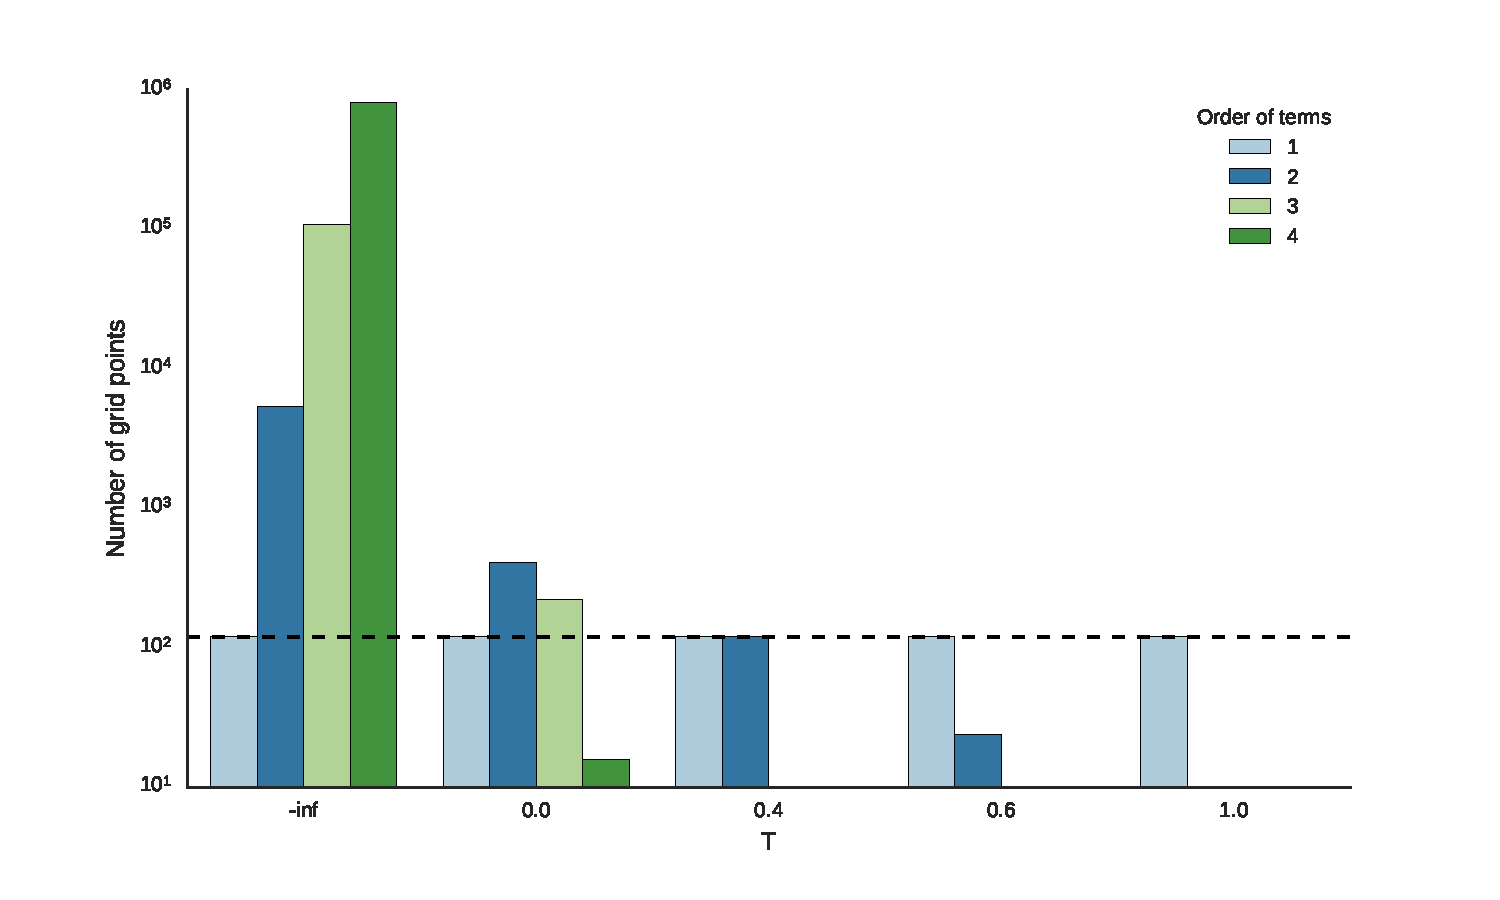
\includegraphics[width=1.2\textwidth]{interactionT}}%
\caption[Order of interaction terms for generalised sparse grids.]{
This figure shows the number of terms of each order for a grid with dimension 4
and level 5.
The bias term is not included in the graphic, it is contained in all grids.}\label{fig:adaptivity}
\end{figure}
Note that the grid for \(T = 1\) does not contain any interaction terms.
The number of grid points of order one, i.e.~points that are constant for all
but one variable stay the same.
The grid for \(T = 1\) does not contain any points except the aforementioned
ones.
\subsection{Results \textit{\&} Discussion}
Generalised sparse grids work well in practice.
We make the following, seemingly obvious hypothesis:
Generalised sparse grids work best, when the interaction terms contain less
information than the grid points of order one.
This is especially important, because sparse grids then allow us to create a
grid with a smaller number of grid points in general, but a higher number of
grid points of order one.

In general the estimated best \(\lambda\) should be smaller for higher values of \(T\) because we perform regularization via discretization for smaller grids, as they have a lower opportunity to capture the training data.
We will test two things in this section:
\begin{enumerate}
\item In what way influences the grid parameter \(T\) the regularization
  parameter \(\lambda\)?
\item Can we archive a better performance with generalised sparse grids compared
  to standard grids, with a comparable number of gridpoints?
\end{enumerate}

We perform a search for \(\lambda\) for the Friedman1 dataset (see \cref{sec:friedman,eq:friedman1}) with identity regularization and a generalized sparse grid for different \(T\)s and level 4.
The results can be seen in the following table:

Before showing some experimental results, we need to look at the relation
between the grid parameter \(T\) and the regularization parameter(s).
Consider the following table, where we perform a search for \(\lambda\) for the
concrete dataset with identity regularization and a generalized sparse grid for
different \(T\)s and level 5.
%Maybe use Mean+-std for cv-grid-size?
\begin{table}[H]
\begin{tabular}[c]{S[table-format=2.1]rS[table-format=2.1]S[table-format=2.6]S[table-format=2.1]rrS[table-format=2.3]S[table-format=2.3]}
  \toprule \multicolumn{1}{r}{\(T\)}
& \multicolumn{1}{r}{\(\Exp[\vert V^T_n \vert]\)}
& \multicolumn{1}{r}{\(\sigma[\vert V^T_n] \vert\)}
& \multicolumn{1}{r}{\(\lambda\)}
& \multicolumn{1}{r}{CV-MSE}
& \multicolumn{1}{r}{Train-Grid}
& \multicolumn{1}{r}{Train-MSE}
& \multicolumn{1}{r}{Test-MSE}
\\\midrule
-0.4 & 8468.7 & 20.60 & 0.01928 & 22.116 & 8470.0 & 5.174 & 17.763\\
0 & 6678.3 & 27.08 & 0.01962 & 22.175 & 6650.0 & 5.227 & 17.508\\
0.5 & 1140.4 & 23.88 & 0.00629 & 22.761 & 1180.0 & 7.099 & 14.414\\
0.6 & 712.7 & 24.21 & 0.01270 & 22.855 & 685.0 & 11.545 & 18.556\\
1 & 517.9 & 23.32 & 0.01015 & 24.300 & 516.0 & 13.162 & 20.318\\
\bottomrule
\end{tabular}
\caption[T vs \(\lambda\)]{Best results and used \(\lambda\) for different
  \(T\)s}\label{fig:t-vs-mse}
\end{table}

We can see a trend in \cref{fig:t-vs-mse}, but the available data is not exhaustive enough to verify this theory.
Note that there is a correlation between grid size and the errors: larger grids
perform better, at least for the cross validation and training error metrics.
This trend will hold for larger levels and smaller \(T\)s at least for the
train-MSE.\@
The cross validation performance will probably not decrease, we can expect diminishing returns at least, until we reach a discretization resolution that leads to severe overfitting.
We can also see that decrease in error between the largest grid and the standard
sparse grid is rather small, considering the amount of additional grid points needed.
The difference between the testing and cross validation error could be reversed
as well, it is difficult to see which method performs better.

\todo{Actually make the comparison here\ldots}
If we compare the performance of the generalised sparse grid with level five and
\(T = 0.5\) with the standard sparse grid of level four, we can see that the
generalised grid performs better than the standard grid, even though they both
use a similair number of grid points.
We can conclude, that our method works well for this dataset, we are able to
archive better results with the same order of grid points.

As an additional result, generalized sparse grids combined with the diagonal
matrix regularization functional performs even better, archiving \ldots.

\section{Interaction-Term Aware Sparse Grids}
Consider a dataset with two features \(x_1\) and \(x_2\).
A sparse grid model of level 3 included not only the bias and the individual
variables, it also includes the interaction term \(x_1 \cdot x_2\).
We call these kind of interactions between two variables two-way interaction,
the one between three variables three-way interaction, and so on.
The interaction terms discussed here are identical to the groups introduced in
the grouped lasso section.

The number of included terms for a \(d\)-dimensional dataset
discretized using a sparse grid of level \(l\) is given by:
\begin{equation*}
  \operatorname{count-terms}(d, l) = \sum_{k  = 0}^{\max (d, l-1)} \binom{d}{k} 
\end{equation*}

%%% Local Variables:
%%% mode: latex
%%% TeX-master: "../main"
%%% End:
